\documentclass[8pt]{extarticle}
\title{}
\author{Avinash Iyer}
\date{}

%font setup
%
%\usepackage[math]{anttor}

%paper setup
\usepackage{geometry}
\geometry{letterpaper, portrait, margin=1in}
\usepackage{fancyhdr}

%symbols
\usepackage{amsmath}
\usepackage{amssymb}
\usepackage{hyperref}
\usepackage{gensymb}

\usepackage[T1]{fontenc}
\usepackage[utf8]{inputenc}

%chemistry stuff
\usepackage[version=4]{mhchem}
\usepackage{chemfig}

%plotting
\usepackage{pgfplots}
\usepackage{tikz}

%\usepackage{natbib}

%graphics stuff
\usepackage{graphicx}
\graphicspath{ {./images/} }

%a useful command
\newcommand{\plain}[1]{\textrm{#1}}

%code stuff
%when using minted, make sure to add the -shell-escape flag
%you can use lstlisting if you don't want to use minted
%\usepackage{minted}
%\usemintedstyle{pastie}
%\newminted[javacode]{java}{frame=lines,framesep=2mm,linenos=true,fontsize=\footnotesize,tabsize=3,autogobble,}
%\newminted[cppcode]{cpp}{frame=lines,framesep=2mm,linenos=true,fontsize=\footnotesize,tabsize=3,autogobble,}

\usepackage{listings}
\usepackage{color}
\definecolor{dkgreen}{rgb}{0,0.6,0}
\definecolor{gray}{rgb}{0.5,0.5,0.5}
\definecolor{mauve}{rgb}{0.58,0,0.82}

\lstset{frame=tb,
	language=Java,
	aboveskip=3mm,
	belowskip=3mm,
	showstringspaces=false,
	columns=flexible,
	basicstyle={\small\ttfamily},
	numbers=none,
	numberstyle=\tiny\color{gray},
	keywordstyle=\color{blue},
	commentstyle=\color{dkgreen},
	stringstyle=\color{mauve},
	breaklines=true,
	breakatwhitespace=true,
	tabsize=3
}
\pagestyle{fancy}
\fancyhf{}
\rhead{Avinash Iyer, Toby Jorgensen}
\lhead{Lab 1}
\begin{document}
\section*{Experiment 1: Evaluating Uncertainties}
\subsection*{Part 1: Measurement of the diameter of a coin}
\begin{quote}
	(1) Measure a diameter of the coin using a meter stick and determine the uncertainty in your measurement. Write down the result in an appropriate format as shown below. Both the best estimate and the uncertainty should have the correct number of decimal places and significant figures.
\end{quote}
\[ d = 19.0 \pm 0.5 \plain{mm} \]
\begin{quote}
	(2) Measure the diameter using a caliper (see Appendix A: How to Use a Vernier Caliper) and report the result in the space below
\end{quote}
\[ d = 19.00 \pm 0.05 \plain{mm} \]
\begin{quote}
	(3) According to the classification given in the Introduction, what kind of uncertainty have you experienced in the above measurements? Explain how you quantified these uncertainties.
\end{quote}
The primary source of uncertainty in measuring the diameter of a coin is instrumental uncertainty from the meterstick and vernier calipers. We quantified the instrumental uncertainty by using the classification used in the introduction — namely, that a meterstick has uncertainty of 0.5mm and the vernier calipers have uncertainty of 0.05mm.
\begin{quote}
	(4) Compare the two measurements taken at steps 1 and 2. Are they consistent within their uncertainties? Explain why or why not.
\end{quote}
They are consistent with the respective uncertainties, we found that for both the vernier calipers and the meterstick, the measurements were around the same value of 19mm, give or take.
\begin{quote}
	(5) Calculate and report fractional uncertainties for both diameter measurements.
\end{quote}
\begin{align*}
	d_1 &= 19.0 \pm 0.5\plain{mm}\\
	&= 19.0 \pm \frac{0.5\plain{mm}}{19.0\plain{mm}}\times100\%\\
	&= 19.0 \pm 3\%\\
	d_2 &= 19.00 \pm 0.05 \plain{mm}\\
	&= 19.00 \pm \frac{0.05\plain{mm}}{19.00\plain{mm}}\times 100\%\\
	&= 19.00 \pm 0.3\%
\end{align*}
\begin{quote}
	(6) Which method is more precise, i.e. has a smaller fractional uncertainty?
\end{quote}
The vernier calipers are more precise as their fractional uncertainty is 1/10 that of the meterstick.
\subsection*{Part 2: Measurement of the diameter of a ping pong ball}
\begin{quote}
	(1) Measure a diameter of the ball using a meter stick. 
\end{quote}
\begin{quote}
	(a) Are you able to determine the diameter to the nearest 1 mm?
\end{quote}
No.
\begin{quote}
	(b) What factor(s) limit your ability to determine the diameter? Clearly state and classify the source(s) of uncertainty in the measured value.
\end{quote}
Random uncertainty and the problem of definition are the most likely sources of uncertainty in attempting to measure the ping pong ball's diameter to the nearest millimeter.
\begin{quote}
	(c) Realistically estimate the uncertainty in your measurement. Can you ignore the instrumental uncertainty of a meter stick? Describe your reasoning in detail.
\end{quote}
The uncertainty in the measurement is likely upwards of 2mm when one includes the random uncertainty and the problem of definition — ignoring the instrumental uncertainty is likely okay because the uncertainties from random uncertainty and the problem of definition are of a larger order of magnitude.
\begin{quote}
	Report the result of your measurement along with the uncertainty in an appropriate format.
\end{quote}
\[ d = 36 \pm 2\plain{mm} \]
\begin{quote}
	(2) Measure the diameter using a caliper. State the source(s) of uncertainty. Report the result of the measurement along with the uncertainty in an appropriate format.
\end{quote}
The primary source of uncertainty is instrumental uncertainty.
\[ d = 39.3 \pm 0.1\plain{mm} \]
\begin{quote}
	(3) Compare the two measurements. Are they consistent within their uncertainties? 
\end{quote}
They are not consistent in their uncertainties, the estimate from the meterstick was significantly lower than the estimate from the caliper.
\begin{quote}
	Calculate and compare the fractional uncertainties and draw a conclusion about the precision of the measurements. 
\end{quote}
\begin{align*}
	d_1 &= 36 \pm 2\plain{mm}\\
	&= 36 \pm \frac{2\plain{mm}}{36\plain{mm}}\times 100\%\\
	&= 36\pm 5\%\\
	d_2 &= 39.3\pm 0.1\plain{mm}\\
	&= 39.3\pm \frac{0.1\plain{mm}}{39.3\plain{mm}}\times 100\%\\
	&= 39.3\pm 0.3\%
\end{align*}
\subsection*{Part 3: Measurement of the diameter of a juggling ball}
\begin{quote}
	(1) State and classify the sources of uncertainty in the diameter measurement. 
\end{quote}
Problem of definition and random uncertainty are the primary sources of uncertainty in the diameter measurement.
\begin{quote}
	(2) Describe in detail how you can estimate the uncertainty in the diameter caused by the problem of definition (remember the solution of Problem 4 in your pre-lab).
\end{quote}
Take multiple measurements of the object, average out the results of the measurement, and the uncertainty will be half the difference between the maximum and minimum values.
\begin{quote}
	(3) Measure the diameter using a meter stick. Show your work and report the final value along with the uncertainty in an appropriate format.
\end{quote}
\begin{align*}
	d_1 &= 49\plain{mm}\\
	d_2 &= 52\plain{mm}\\
	d_3 &= 53\plain{mm}\\
	d &= \plain{avg}(d_1,d_2,d_3) \pm 2\plain{mm}\\
	&= 51 \pm 2\plain{mm}
\end{align*}
\begin{quote}
	(4) Measure the diameter using a caliper. Show your work and report the final value along with the uncertainty in an appropriate format.
\end{quote}
\begin{align*}
	d_1 &= 52.6 \pm 0.1\plain{mm}\\
	d_2 &= 52.3 \pm 0.1\plain{mm}\\
	d_3 &= 51.6 \pm 0.1\plain{mm}\\
	d &= 52.2 \pm 0.5\plain{mm}
\end{align*}
\begin{quote}
	(5) Compare the two measurements. Are they consistent within the uncertainties? 
\end{quote}
Yes, these measurements and uncertainties are consistent.
\begin{quote}
	(6) What was a primary source of uncertainty for measuring the diameter with a meter stick? With a caliper?
\end{quote}
The primary source of uncertainty with the meter stick was the problem of definition, while the primary source of uncertainty with the caliper was instrumental uncertainty.
\begin{quote}
	(7) Does using a caliper instead of a meter stick increase the precision of the measurement? Explain.
\end{quote}
Yes — because the primary source of uncertainty with the caliper, instrumental uncertainty, is much lower than uncertainty from the problem of definition.
\section*{Experiment 2: Graphing, Error Bars, and Uncertainty in Slope}
\begin{quote}
	(1)Assuming that the car moves at constant velocity, what kind of graph do you expect to produce when plotting Distance vs. Time?  Predict the graph’s intercept.
\end{quote}
Assuming the car moves at constant velocity, the graph of distance vs. time would be a straight upward sloping line with intercept at zero.
\begin{quote}
	(2) How will you obtain the speed using the graph?
\end{quote}
We'll get the speed from the graph by taking the change in distance over the change in time over the measurement period.
\begin{quote}
	(3) Do you expect that all of the data points will lie exactly on the predicted line?  Explain.
\end{quote}
No, because there will be uncertainty in the time at which the measurement takes place as well as uncertainty in the measurement itself.
\begin{quote}
	(4) Using a colored tape, set six marks spaced 0.5 m apart in a straight line. You will measure time intervals over which the car travels various distances, and estimate uncertainties in your measurements as follows:
	
	Uncertainty in time measurement. This uncertainty is caused by your ability to turn on and off a stopwatch just at the right moments of time rather than by the accuracy and precision of the instrument. Suppose you can press the button within 0.2 s of either the start (t1) or stop (t2) of the measurement. So t1 = t1 best ± 0.2 s and t2 = t2 best ± 0.2 s. The highest value for the time interval t = t2 - t1 is t2 bes - t1 best + 0.4 s (when t1 has its smallest value and t2 has its largest value), and the lowest value is t2 bes - t1 best - 0.4 s (when t1 has its largest value and t2 has its smallest value). Thus, the uncertainty in t is δt = 0.4 s. Using this line of reasoning, we overestimated the uncertainty δt, but that is ok for now. 
	
	Uncertainty in distance measurement. The precision of the distance measurement is actually very high (small uncertainty is caused by the precision of the tape measure and possible slight deviation of the car from the line parallel to the tape measure). However, for educational purposes, we will suppose the uncertainty in distance δx is equal to 0.1 m. Although this is obviously a gross overestimation, it is ok for now.
	
	Notice that both δt and δx remain the same for all the measurements.
	
	Perform the experiment for the distances shown in the table below. Take a single measurement of t for each distance and record your results in the table.
\end{quote}
\begin{center}
	\begin{tabular}{c|c}
		$t \pm 0.4s$ & $x \pm 0.1m$\\
		\hline
		1.4 & 0.5\\
		2.5 & 1.0 \\
		3.7 & 1.5\\
		4.9 & 2.0\\
		6.2 & 2.5
	\end{tabular}
\end{center}
\begin{quote}
	(5) Plot the data on a scatter plot (without a best-fit line) in Excel and represent the uncertainties graphically using horizontal and vertical error bars (see the Excel Manual for instructions on how to create graphs and add error bars). Be sure that your graph is titled and that the axes are properly labeled. Include the graph in the space below. Note that tables and graphs must always be included in the body of a Lab Report at an appropriate location.  Do not simply attach tables and graphs to the end of a Lab Report. Does the graph look like a linear relationship?
\end{quote}
\begin{center}
	\resizebox{10cm}{!}{
	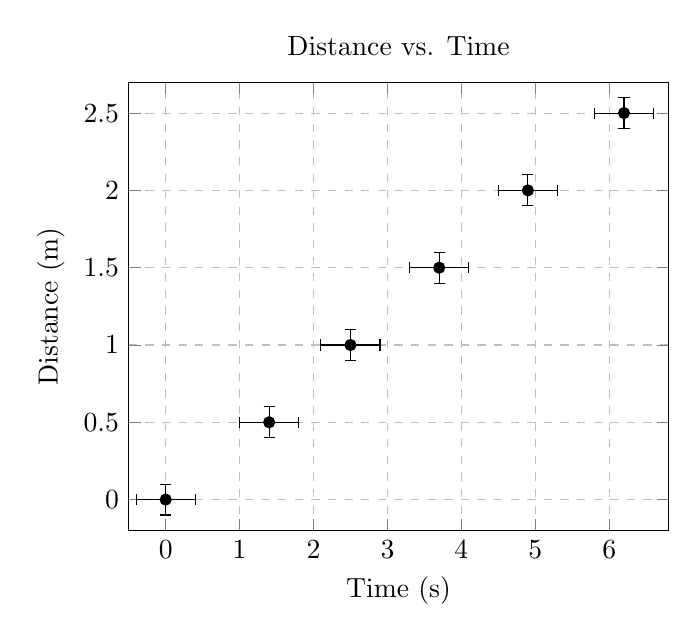
\begin{tikzpicture}
		\begin{axis}[
			title={Distance vs. Time},
			xlabel={Time (s)},
			ylabel={Distance (m)},
			xmin = -0.5, xmax = 6.8,
			ymin=-0.2, ymax = 2.7,
			xtick={0,1,2,3,4,5,6},
			ytick={0,0.5,1,1.5,2,2.5},
			xmajorgrids=true, ymajorgrids=true, grid style = dashed,
			]
			\addplot[only marks, error bars/.cd, y dir = both, x dir = both, x explicit, y explicit] coordinates {
				(0,0) +- (0.4,0.1)
				(1.4,0.5) +- (0.4,0.1)
				(2.5,1.0) +- (0.4,0.1)
				(3.7,1.5) +- (0.4,0.1)
				(4.9,2.0) +- (0.4,0.1)
				(6.2,2.5) +- (0.4,0.1)
			};
		\end{axis}
	\end{tikzpicture}
	}
\end{center}
\begin{quote}
	(6) On the printed graph above, draw (by hand) the line that you think best fits the data points.  Explain how and why you have drawn this line. Note that there is an implicit data point for time of zero and distance of zero at the origin. Your best-fit line should pass through this point.
\end{quote}
\begin{center}
	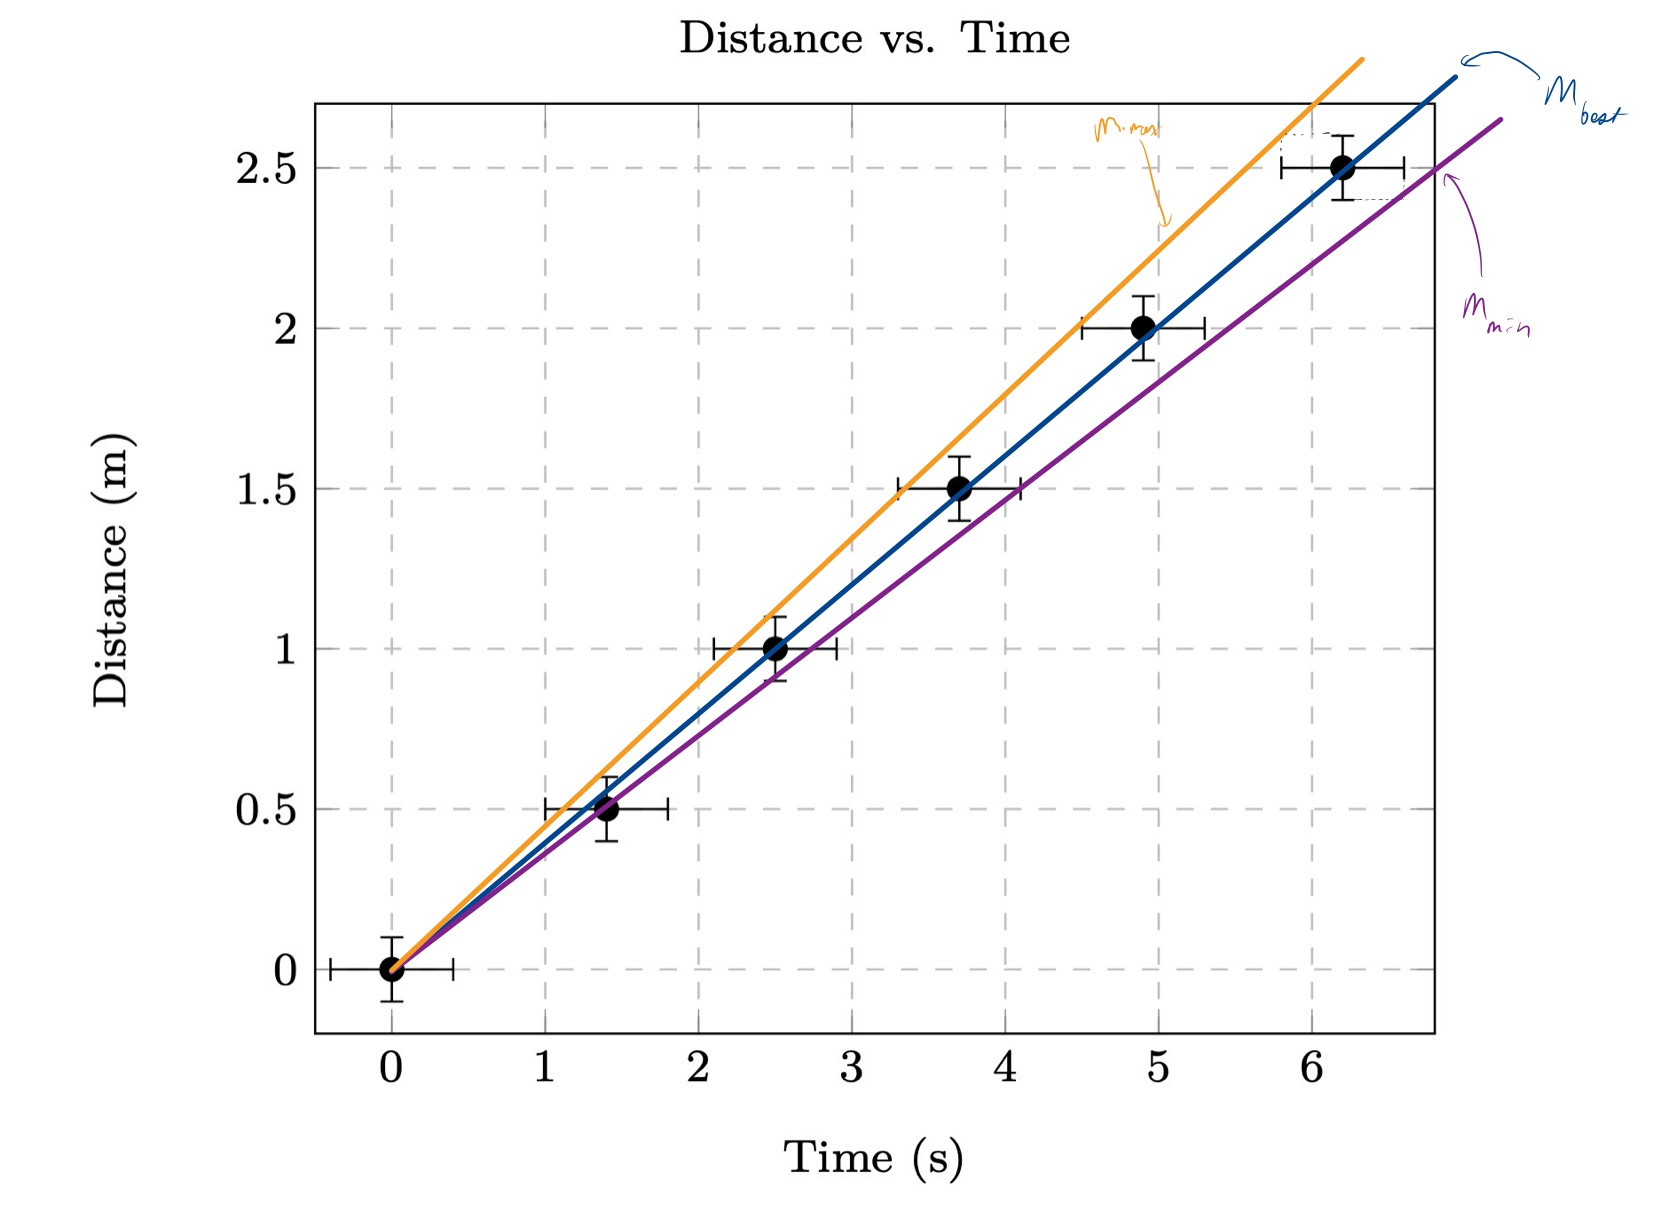
\includegraphics[width=10cm]{Lab1Image1_2}
\end{center}
\noindent We drew the best fit line by attempting to minimize the deviation it had from the various points while staying within the uncertainty boxes of each one.
\begin{quote}
	(7) Measure and report the speed using your best-fit line. List the coordinates of the used points, and show your calculations. (Hint: Minor horizontal and vertical gridlines in the chart will help you!)
\end{quote}
\begin{align*}
	m_{\plain{best}} &= \frac{2.5-0.0}{6.2-0.0} \\
	&= 0.40~\plain{m/s}
\end{align*}
We used the coordinates from $(6.2,2.5)$ as using it led to the least deviation from the rest of the points.
\begin{quote}
	(8) On the printed graph above, draw the "min" line - the one with the smallest slope that you can draw through the data points within the uncertainties. \textbf{Note that the line should not necessarily pass through or touch all the error bars; it should rather pass through or touch the \underline{uncertainty rectangle} about every point (see figure below)}. Measure and report the slope of this line. List the coordinates of the used points, and show your calculations.  
\end{quote}
\begin{align*}
	m_{\plain{min}} &= \frac{2.4-0.0}{6.6-0.0}\\
	&= 0.36~\plain{m/s}
\end{align*}
We used the point $(6.6,2.4)$, which represents the maximum negative uncertainty vertically and maximum positive uncertainty horizontally from the point at $(6.2,2.5)$ while still touching all the error boxes.
\begin{quote}
	(9) In the same way, draw the "max" line -- the one with the largest slope that you can draw through the datapoints within the uncertainties. Measure and report the slope of this line. List the coordinates of the used points, and show your calculations.  
\end{quote}
\begin{align*}
	m_{\plain{max}} &= \frac{2.6-0.0}{5.8-0.0}\\
	&= 0.45~\plain{m/s}
\end{align*}
We used the coordinate $(5.8,2.6)$, which represents the maximum positive uncertainty from $2.5$ and maximum negative uncertainty horizontally from $6.2$.
\begin{quote}
	(10) Calculate and report the uncertainty in the slope as one-half of the difference between max and min slopes. Note that the best fit may not lie exactly half way between the two worst fits.
\end{quote}
\begin{align*}
	\delta x &= \frac{m_{\plain{max} - m_{\plain{min}}}}{2} \\
	&= \frac{0.45 - 0.36}{2} \\
	&= 0.05~\plain{m/s}
\end{align*}
\begin{quote}
	(11) Report the value for the speed along with the uncertainty in an appropriate format.
\end{quote}
\[ v = 0.40 \pm  0.05~\plain{m/s}\]
\begin{quote}
	(12) If the distance range was smaller, would the uncertainty in speed be smaller, larger or remain the same? Explain. 
\end{quote}
If the distance range were smaller, the uncertainty in speed would be smaller as the difference between maximum and minimum possible distance would shrink the maximum and minimum possible speed, all else equal. For example, if the distance range is $\pm 0.1$, the speed at time $t$ with distance $d$ would be $\frac{d}{t} \pm \frac{0.1}{t}$, but if the distance range were $\pm 0.01$, then the speed at time $t$ with distance $d$ would be $\frac{d}{t} \pm \frac{0.01}{t}$, which is lower.
\end{document}
